\section{Modifiche allo Splice-Aware Aligner}
Lo Splice-Aware Aligner svolge due compiti:
\begin{enumerate}
	\item Generazione dello Splicing Graph e della sua Linearizzazione
	\item Allineamento delle read di RNA-Seq alla Linearizzazione dello Splicing Graph
\end{enumerate}
L'allineamento avviene utilizzando il concetto di MEM (Maximum Exact Matching); l'output verrà convertito in formato SAM per permettere l'eventuale elaborazione con altri strumenti.

\subsection{Allineamento di entrambe le read}
Il primo problema da affrontare è ovviamente il fatto che sia ora necessario allineare due read e non una; fortunatamente si tratta solo di iterare il processo di allineamento su una coppia di read ad ogni ciclo, anziché su read singola. Verranno quindi generati due file contenti MEM anziché uno. Sarà poi compito della Formattazione SAM "fondere" i due file MEM per ottenere un SAM Completo.

\subsection{Introduzione di read unmapped e "placeholder" nel formato MEM}
Nei file MEM ottenuti dallo Splice-Aware Aligner vengono ora visuallizati due nuovi tipi di MEM: quelli relativi alle read unmapped e quelli relativi ai "placeholder". Il primo caso è banale, e rappresenta tutte quelle read che non hanno un matching esatto di lunghezza considerevole con il genoma dato in input.
Il secondo caso è più complesso e rappresenta un insieme di read fasulle utilizzate solo come padding per avere due file MEM della stessa lunghezza: questo facilita enormemente l'elaborazione nello step successivo (la formattazione SAM). Come detto in precedenza quando si lavora con read paired-end è sempre necessario lavorare a coppie, ma non sempre ad uno stesso pair è associato lo stesso numero di allineamenti secondari: è qui che entrano in gioco i "placeholder". La loro implementazione è banale: si tengono due contatori (che rappresentano rispettivamente il numero di allineamenti relativi alla prima read e quelli relativi alla seconda read), si ottengono separatamente gli allineamenti relativi a ciascuna delle due read, e si controllano i contatori. Si prende il minore dei due e si aggiungono tanti placeholder quanto bastano per rendere uguali i contatori.

\begin{algorithm}
\caption{Algoritmo per l'aggiunta dei placeholder}\label{placeholder}
\begin{algorithmic}[1]
%\Procedure{addPlaceholders}{}
	\State $count\_aligns\_1 \gets 0, count\_aligns\_2 \gets 0$
	\While{$count\_aligns\_1 != count\_aligns\_2$}
		\If{$count\_aligns\_1 < count\_aligns\_2$}
			\State $addPlaceholder(file1)$
			\State $count\_aligns\_1++$
		\Else
			\State $addPlaceholder(file2)$
			\State $count\_aligns\_2++$
		\EndIf
	\EndWhile\label{euclidendwhile}
	%\EndProcedure
\end{algorithmic}
\end{algorithm}

\begin{figure}[h]
	\centering
	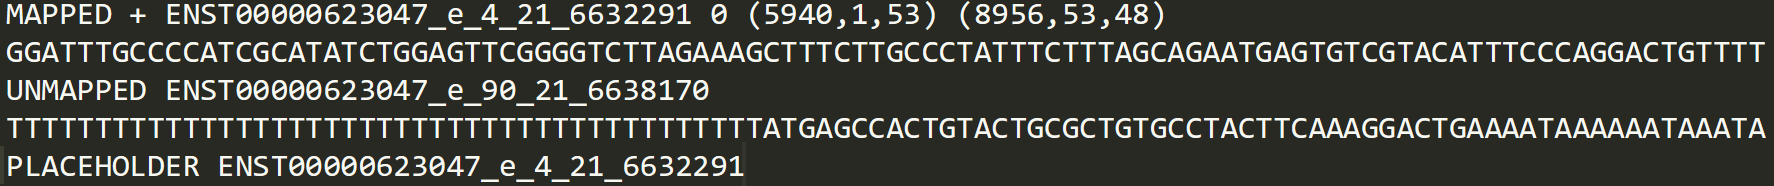
\includegraphics[width=\linewidth]{images/tipiMEM2.png}
  \caption{I diversi tipi di MEM}
  \label{fig:AlternativeSplicingTypes}
\end{figure}

\subsection{Supporto alle fragment library types}

